\documentclass[11pt,a4paper]{article}

%
% $Id: userguide.tex 526 2007-10-31 08:57:09Z schnelle $
%

\usepackage[latin1]{inputenc}
\usepackage{graphics}
\usepackage{graphicx}
\usepackage{url}
\usepackage{listings}
\usepackage{xcolor}
\usepackage{jvoicexml}

\newcommand{\speech}[2]{\noindent\hangindent=\parindent{\textbf{#1:}} #2\par}

\title{JVoiceXML 0.7.2 User Guide}
\version{0.7.2}
\author{Dr. Dirk Schnelle-Walka}
\email{dirk.schnelle@jvoicexml.org}
\date{\today}

\begin{document}
\pagestyle{empty}
\lstset{language=Java,language=XML,
        backgroundcolor=\color{lightgray},
        basicstyle=\small,
        numbers=left,
        numberstyle=\tiny,
        stepnumber=5}

\maketitle

\pagestyle{headings}

\tableofcontents

\newpage

\begin{abstract}
This documents describes the API of JVoiceXML from the user's point of
view. It provides information about the coding of clients for
the JVoiceXML voice browser.
\end{abstract}


\section{Introduction}
\label{sec:introduction}

JVoiceXML is a free VoiceXML~\cite{w3.org:voicexml} implementation written in 
the JAVA programming language with an open architecture for custom
extensions. It offers a library for easy VoiceXML
document creation and a VoiceXML interpreter to process 
VoiceXML documents.Demo implementation platforms are supporting JAVA standard
APIs such as JSAPI~\cite{sun:jsapi} and JTAPI~\cite{sun:jsapi}.

JVoiceXML is hosted at SourceForge~\cite{sourceforge} as an open source project.
You find everything that is related to this project under
\url{http://sourceforge.net/projects/jvoicexml/}.
The work on the browser is still in progress and not all tags are
supported, yet. You are invited to help us finishing the work to make this
project a success.

This document provides information about the installation and
configuration of the JVoiceXML voice browser and how to write
VoiceXML applications for this browser.
It is assumed that readers are familiar with the concepts of
VoiceXML and Java programming.

This document refers to UNIX and Windows systems. JVoiceXML will work with 
any other operating systems that support Java 6, too.

Nobody is perfect, so you may find some errors or small things to correct.
Please let me know if you think you found something that should be written
differently or should be added.

\section{Copyright}
\label{sec:copyright}

JVoiceXML uses the GNU library general public license~\cite{gnu:lgpg}. 
This is mentioned in all our source files as a unique header.
You can find a copy in the file COPYING in the \$\{JVOICEXML\_HOME\}
directory. This means that you are allowed to use JVoiceXML
library in your commercial programs. If you make some nice
enhancements it would be great, if you could send us your
modifications so that we can make it available to the public.

JVoiceXML is free software; you can redistribute it and/or
modify it under the terms of the GNU Library General Public
License as published by the Free Software Foundation; either
version 2 of the License, or (at your option) any later version.

JVoiceXML is distributed in the hope that it will be useful,
but WITHOUT ANY WARRANTY; without even the implied warranty of
MERCHANTABILITY or FITNESS FOR A PARTICULAR PURPOSE. See the GNU
Library General Public License for more details.

You should have received a copy of the GNU Library General Public
License along with this library; if not, write to the Free
Foundation, Inc., 59 Temple Place, Suite 330, Boston, MA  02111-1307  USA

\section{Architectural Overview}
\label{sec:arch-overv}

Before going into detail the general architecture and concepts are presented.
The basic architecture is shown in figure~\ref{fig:architecture}.

\begin{figure}
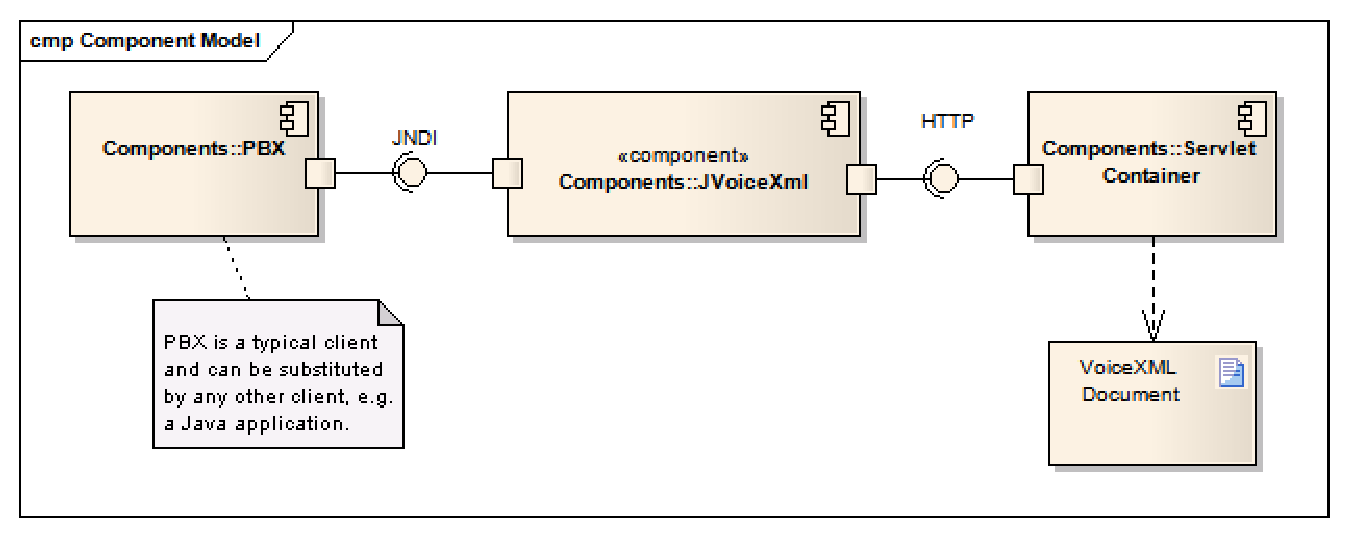
\includegraphics[width=\linewidth]{architecture.eps}
\caption{Basic architecture of JVoiceXML}
\label{fig:architecture}
\end{figure}

The VoiceXML documents are stored in a web server or a servlet container
and are accessed, e.g., via the HTTP protocol.
JVoiceXML runs as a standalone server and retrieves the documents from
the servlet container. 

Clients use the Java Naming and Directory Interface (JNDI)~\cite{sun:jndi} to 
access JVoiceXML. They can also initiate calls for an application using this 
technology. Currently there is no telephony support, but users can call 
applications from their own Java programs. The way this is done is described in
the following sections.

Conceptually JNDI allows to connect to a centralized running JVoice\-XML 
server. However this does not make much sense for the current demo 
implementation, since the speaker and the microphone of the JVoiceXML server
is used for speech output and input.

\section{Required Software}
\label{sec:required-software}

JVoiceXML is written in JAVA and you will at least need a JAVA compiler, an 
editor or preferably a JAVA IDE, see section~\ref{sec:ide}, and ANT, see 
section~\ref{sec:ant}, to run the browser and build the binaries for the 
clients. Tomcat~\cite{apache:tomcat} from the Apache Software Foundation can be
used as a servlet container.

\subsection{IDE}
\label{sec:ide}

You can use the IDE of your choice to edit the sources and compile the 
demos. You can even use a simple text editor to perform this job.
Nevertheless there are some restriction that you cannot work around.

Your IDE must support at least J2SE 1.6. The demos use ANT 1.7 for compilation. 
ANT is not required but used as a means of IDE independent project setup.

\subsection{JAVA}
\label{sec:java}

Parts of the code of JVoiceXML are using features from the JAVA 5 API, so that
you will need at least J2SE 1.6 to compile the code. You can download it
for free from \url{http://java.sun.com}.

\subsection{ANT}
\label{sec:ant}

The demos are being built by an ANT build file to keep it IDE independent. It is
recommended that you use at least ANT 1.7.0. 
If you don't have ANT installed, you can download the current release
from \url{http://ant.apache.org}.

Nearly all IDEs feature an ANT integration. This allows to use the scripts with
your favorite IDE.

\subsection{Tomcat}
\label{sec:tomcat}

VoiceXML is designed to access documents via the HTTP protocol among others. This
guide uses Tomcat 5.5~\cite{apache:tomcat} for this purpose.
 Tomcat can be obtained
from \url{http://tomcat.apache.org}. You can also use the servlet container of
your choice.


\section{Installation}

You can download the compiled voice browser as \texttt{jvxml-VERSION.zip} from 
\url{http://jvoicexml.sourceforge.net/downloads.htm}.
\texttt{VERSION} has to be replaced by the used version number, e.g. 0.7.0.GA.
Unpack the zipped distribution file and open a command prompt in that
directory. Call the installer 

\begin{lstlisting}
java -jar jvxml-install-VERSION.jar
\end{lstlisting}

For windows double-clicking the jar should do the trick. 

This will install the browser into a directory of your choice. In the rest of 
this document this directory will be referred as \lstinline{JVOICEXML_HOME}.

JVoiceXML is shipped with different implementation platforms. Install only
those platforms that you intend to use. The configuration issues of each
platform is described in the following sections.

It is also possible to install everything and drop those configuration files
from the \lstinline{$JVOICEXML_HOME/config} folder that you do not need. You
can simply create a subfolder \lstinline{unused} in that directory and move the
unused configuration files to this folder. The configuration files follow the
naming convention \lstinline{<platform>-implementation.xml}. The following
section gives a first insight into the overall configuration concept.

\subsection{Implementation Platform Configuration}
\label{sec:impl-platform-config}

With the release of JVoiceXML 0.7.0.GA a new configuration concept was
introduced which allows for a more flexible and modular configuration. Each
implementation platform can add custom libraries without the need to adapt the
startup script. The following code snippet shows the configuration of the text
based implementation platform.

\begin{lstlisting}[language=XML]
<?xml version="1.0" encoding="UTF-8"?>
<implementation
  xmlns:beans="http://www.springframework.org/schema/beans"
  xmlns:xsi="http://www.w3.org/2001/XMLSchema-instance"
  xsi:noNamespaceSchemaLocation=
    "jvxml-implementation-0-7.xsd">
  <classpath>lib/jvxml-text.jar</classpath>
  <classpath>lib/jvxml-client-text.jar</classpath>
  <beans:bean class=
    "org.jvoicexml.implementation.text.TextPlatformFactory">
    <beans:property name="instances" value="1" />
  </beans:bean>
</implementation>
\end{lstlisting}

The configuration introduces two new Java archives to the classloader:
\lstinline{ib/jvxml-text.jar} and \lstinline{ib/jvxml-client-text.jar}.

\subsubsection{Classloader repositories}

The Java archives that are introduced by the configuration are loaded in isolated
classloader repositories. Java regards two classes to be different if they are
loaded from different classloaders these libraries must share the same
classloader. On the one hand this is an advantage since it offers the opportunity
to have different versions of the same library active in different classloader
repositories, on the other hand this can be a drawback since we want to share the
libraries among different configuration settings, e.g. a callmanager
configuration and an implementation platform configuration. Sharing the same
classloader repository can be achieved by adding the following line to the
configuration file

\begin{lstlisting}[language=XML]
<repository>name</repository>
\end{lstlisting}

\emph{name} should be replaced a proper name for the repository, e.g.
\emph{text} for the text based implementation platform.

A closer look at certain configuration issues is given in
section~\ref{sec:configuration}.

\subsection{JSAPI 1.0 implementation platform}

The JSAPI 1.0 implementation platform targets JSAPI 1.0 compliant speech
recognizers and synthesizers. As a first start JVoiceXML is shipped with Sphinx
4 and FreeTTS.

It is also possible to use other speech recognizers and synthesizers. An
example how to enable Talking Java for JVoiceXML is described in
section~\ref{sec:talking-java}.

\subsection{JSAPI 2.0 implementation platform}

The JSAPI 2.0 implementation platform targets JSAPI 2.0 compliant speech
recognizers and synthesizers. As a first start JVoiceXML is shipped with a
first approach to use Sphinx 4 and FreeTTS with this new API.

This is an implementation of a draft specification developed under the Java
Community Process (JCP) and is made available for testing and evaluation
purposes only. The code is not compatible with any specification of the JCP.

Note that you still need to download \lstinline{jsapi2.jar} from
\url{http://www.conversations.com} and copy it to the
\lstinline{$JVOICEXML_HOME/lib} folder. Otherwise you will get an exception
when you start the voice browser.

\subsection{JTAPI implementation platform}

The JTAPI implementation platform can be used in addition to any other
implementation platform to enable telephony support. Currently there are some
basic tests with the JSAPI 2.0 implementation platform, but this one needs some
more programming.

\subsection{MRCPv2 implementation platform}

The MRCPv2 implementation platform targets MRCPv2 compliant speech recognizers
and synthesizers. This platform is useful, if you are interested in an easy
integration with commercial server based speech engines. Unfortunately it is
currently not working. If you are not interested in debugging of this
implementation platform it is recommended to remove this configuration file from
the config folder.

\subsection{Text implementation platform}

The text implementation platform can be used to have a string based access to
the voice browser.

\section{Starting the Voice Browser}

After the installation, the browser is ready to use. 
The \texttt{bin} folder contains the files to start the browser. The relevant
files depend on your operating system and are described in the following
sections.

Make sure that you have your configuration right as described in
section~\ref{sec:impl-platform-config} and that you downloaded and installed
the missing jars if applicable.

Having started the voice browser it is waiting for incoming requests from a
client. Later on in this guide we wil explain how to code such a client.

\subsection{Linux}

The shell script \texttt{startup.sh} located in the \texttt{bin} folder
of your JVoiceXML installation can be used to start the browser.

It is written to work independent to the current folder. Simply call

\begin{lstlisting}
sh JVOICEXML_HOME/bin/startup.sh
\end{lstlisting}

After the start lots of debug information will be displayed.
It may take a while until the TTS engine and the recognizer are launched.
The voice browser can be used, if you see the message

\begin{lstlisting}
VoiceXML interpreter <version> (Build <number>) started.
\end{lstlisting}

\subsection{Windows}

The windows executable \texttt{JVoiceXML.exe} located in the \texttt{bin}
folder of your JVoiceXML installation can be used to start the browser.

The executable is simply a wrapped Java call and should also work with a
double-click in the windows explorer.

From The command line prompt, call

\begin{lstlisting}
JVOICEXML_HOME\bin\JVoiceXML.exe
\end{lstlisting}

If you start the browser from the windows explorer, a command prompt will open.
After the start lots of debug information will be displayed.
It may take a while until the TTS engine and the recognizer are launched.
The voice browser can be used, if you see the message

\begin{lstlisting}
VoiceXML interpreter <version> (Build <number>) started.
\end{lstlisting}

\section{Shutdown of the Voice Browser}

The \texttt{bin} folder also contains the files to stop the browser. The
relevant files depend on your operating system and are described in the following
sections.

Please avoid to stop the browser using \lstinline{CTRL-C} or by closing the
window. If you have JNDI configured JVoiceXML starts the \lstinline{rmiregistry}. The
registry may not shutdown properly if you closed the voice browser this way and may keep the
configured port active. This will result in some error messages if you restart
JVoiceXML.

\subsection{Linux}

The shell script \texttt{stutdown.sh} located in the \texttt{bin} folder
of your JVoiceXML installation can be used to stop the browser.

It is written to work independent to the current folder. Simply call

\begin{lstlisting}
sh JVOICEXML_HOME/bin/shutdown.sh
\end{lstlisting}

This will make an RMI call to the voice browser and asks it to shutdown.

\subsection{Windows}

The windows executable \texttt{Shutdown.exe} located in the \texttt{bin}
folder of your JVoiceXML installation can be used to stop the browser.

The executable is simply a wrapped Java call and should also work with a
double-click in the windows explorer.

From The command line prompt, call

\begin{lstlisting}
JVOICEXML_HOME\bin\Shutdown.exe
\end{lstlisting}

This will make an RMI call to the voice browser and asks it to shutdown.

\section{Running the Demos}

The browser comes with some demo programs. You'll find them in the
directory \texttt{JVOICEXML\_HOME/demo}. Use the IDE of your choice
and explore there contents. Some features of the browser can 
become more clear with them.

The demos are designed to work with the JSAPI 1.0 implementation platform. Make
sure that you have this configuration enabled before running the demos.

The demo programs feature an ANT script which can be used for starting.
There may be some properties that need to be overwritten in the installed
version. For this purpose there is a template \lstinline{ant.properties} of
relevant properties in the folder \lstinline{JVOCEXML_HOME/demo/config-props}.
To override these properties copy the file \texttt{ant.properties} to the
folder \lstinline{JVOCEXML_HOME/demo/personal-props}. This way you are able
to keep the original settings but also override custom values.

In most cases it should be sufficient to change to each demo directory
and call

\begin{lstlisting}
ant run
\end{lstlisting}

The procedure described above will not work for the
\emph{HelloWorldServletDemo}. In this case you have to add the location of
\texttt{servlet-api.jar} to the \texttt{jvoicexml.properties} by adjusting the
property \texttt{servlet.lib.dir}.

Before you can run this demo, call

\begin{lstlisting}
ant war
\end{lstlisting}

to create a war archive that must be deployed to you servlet container
before running the demo.

\section{A first TTS example}
\label{sec:first-tts-example}

This first example shows how VoiceXML documents are accessed from a
servlet container or a web server and how clients can start the application.

It is also possible to have the VoiceXML files in the file system. In this case
you have to use a URL using the \lstinline{file} scheme, e.g.
\lstinline{file:///home/user/text.vxml}. For this guid we follow the W3C
specification to retrieve the VoiceXML documents via the \lstinline{HTTP}
protocol.

\subsection{Creating the VoiceXML file}
\label{sec:hello-vxml}

This first example is very simple. It just echos a 'hello world'.
Create a file \texttt{hello.vxml} with the following content:

\begin{lstlisting}[language=XML]
<?xml version="1.0" encoding="UTF-8"?> 
<vxml xmlns="http://www.w3.org/2001/vxml" version="2.1">
  <form>
    <block>Hello World!</block>
  </form>
</vxml>
\end{lstlisting}

Copy this file to a directory of your web server that can be accessed
by a browser. For Tomcat create a directory \texttt{demo1} in
the \texttt{\$CATALINA\_HOME/web\-apps} directory and copy the VoiceXML
file to this directory. In order to make this
an accessible web application, create the empty sub-folder \texttt{WEB-INF}
in \texttt{demo1}.

Now, try to access the file in your browser. For Tomcat this is
\url{http://localhost:8080/demo1/hello.vxml}. If all went well the
contents of this file is displayed in the browser. In some cases the file
might be offered for download. This is the default behaviour of your browser if
it can not determine the type of the file. Download the file and open it in your
favourite editor to verify that this is your VoiceXML code.

\subsection{Writing the Client}

A client is a program that remotely calls JVoiceXML and initiates calls. Create 
a Java file \texttt{Demo1.java} with the following content:

\begin{lstlisting}[language=Java]
public class Demo1 {
    public static void main(String[] args) {
    }
}
\end{lstlisting}

First, we need to connect to the JVoiceXML voice browser. JVoiceXML
uses JNDI over RMI~\cite{sun:rmi,sun:rmi_jndi} for this purpose. 
The following code snippet
shows how to obtain a remote reference to the main entry for
all client applications \texttt{org.jvoicexml.JVoiceXml}:

\begin{lstlisting}[language=Java]
import javax.naming.Context;
import javax.naming.InitialContext;

import org.jvoicexml.JVoiceXml;
...
    public static void main(String[] args) {
        Context context = null;
        try {
            context = new InitialContext();
        } catch (javax.naming.NamingException ne) {
            ne.printStackTrace();
            System.exit(-1);
        }

        JVoiceXml jvxml = null;
        try {
            jvxml = (JVoiceXml) context.lookup("JVoiceXml");
        } catch (javax.naming.NamingException ne) {
            ne.printStackTrace();
            System.exit(-1);
        }
...
\end{lstlisting}

In line 9, a \texttt{Context} is created to access JNDI resources.
The settings how to do this are obtained from a file named
\texttt{jndi.properties} which is in the \texttt{CLASSPATH}.
\texttt{jndi.properties} has the following contents:

\begin{lstlisting}
java.naming.factory.initial=\
    com.sun.jndi.rmi.registry.RegistryContextFactory
java.naming.provider.url=rmi://localhost:1099
java.naming.rmi.security.manager=true
\end{lstlisting}

The location of JVoiceXML is stored in the property 
\texttt{java.naming.pro\-vider.url}. If you want to access JVoiceXML on a 
different computer you have to replace \texttt{localhost} with the IP address 
or name of that computer.

The classes  that are required to access JVoiceXML, like 
\texttt{org.jvoice\-xml.JVoiceXml}, are part of the
\texttt{jvxml-client.jar} and \texttt{jvxml-xml.jar}, which can be found in the
\texttt{lib} folder of you JVoiceXML installation. This jar contains all classes, that you 
need to write client applications.

If you are using Java 5 you will have to add the Java API for XML streaming.
This became part of Java 6 as JSR 173. These are \texttt{jsr173\_\-1.0.jar} and
\texttt{sjsxp.jar}. You can find a copy of these libraries in the lib folder of your JVoiceXML installation.

Next, we call the browser to process the application. This is done
by creating a \texttt{org.jvoicexml.Session} object.

\begin{lstlisting}[language=Java]
...
import org.jvoicexml.Session;
...

    public static void main(String[] args) {
        ...
        JVoiceXml jvxml = null;
        try {
            jvxml = (JVoiceXml) context.lookup("JVoiceXml");
        } catch (javax.naming.NamingException ne) {
            ne.printStackTrace();
            System.exit(-1);
        }

        final Session session = 
            jvxml.createSession(null);

        final URI uri;
        try {
            uri = 
          new URI("http://localhost:8080/demo1/hello.vxml");
        } catch (URISyntaxException e) {
            e.printStackTrace();
            System.exit(-1);
        }

        try {
            session.call(uri);

            session.waitSessionEnd();

            session.hangup();
        } catch (org.jvoicexml.event.JVoiceXMLEvent e) {
            e.printStackTrace();
            System.exit(-1);
        }
    }
...
\end{lstlisting}

The argument on the \texttt{createSession} method must be 
\texttt{null}. It is reserved for future use, once we have telephony
support. The argument for \texttt{call} must point to to URI of the
root document of your application.

\subsection{Starting the Client}
\label{sec:starting-client}

The JNDI implementation of JVoiceXML is based on RMI, and
the implementation for the used interfaces are obtained by
RMI dynamic code download. This means that you have to provide
the location of the library with the implementation of the
interfaces and a security policy file.

For the start this security policy file \texttt{jvoicexml.policy}
allows everything to the remote user:

\begin{lstlisting}
grant {
    permission java.security.AllPermission;
};
\end{lstlisting}

A more restrictive policy can be

\begin{lstlisting}
grant {
  permission java.util.PropertyPermission
      "jvoicexml.vxml.version", "read";
  permission java.util.PropertyPermission
      "jvoicexml.xml.encoding", "read";
  permission java.net.SocketPermission
      "127.0.0.1:1024-", "connect,resolve";
  permission java.io.FilePermission
      "${JVOICEXML_HOME}/lib/-", "read";
};
\end{lstlisting}

The location of the policy is provided by the following environment property

\begin{lstlisting}
-Djava.security.policy=jvoicexml.policy
\end{lstlisting}

Once you start Demo1 it connects to JVoiceXML and starts processing
the application. If you are successful you should hear a synthesized voice
speaking \emph{Hello World}. The application terminates when the processing
finishes.

\section{Creating VoiceXML using the Tag Library}

JVoiceXML features a strong tag library to author VoiceXML documents. In
this section we will write a small servlet returning the VoiceXML document that
was used in section~\ref{sec:first-tts-example} using this library.

\subsection{Creating the Servlet}

Our basic seleton for a servlet looks as follows:

\begin{lstlisting}
import java.io.IOException;
import javax.servlet.ServletException;
import javax.servlet.http.HttpServlet;
import javax.servlet.http.HttpServletRequest;
import javax.servlet.http.HttpServletResponse;

public class HelloServlet extends HttpServlet {
    public void doGet(HttpServletRequest request,
        HttpServletResponse response)
        throws ServletException, IOException {
    }
}
\end{lstlisting}

Our code goes into the \texttt{doGet()} method of the servlet. The tag library
is located in the package \texttt{org.jvoicexml.xml}. Hence you have to add
\texttt{jvxml-xml.jar} to the CLASSPATH.

Before using the classes you have to import the required classes by adding
\begin{lstlisting}
import org.jvoicexml.xml.*;
\end{lstlisting}

Then, the VoiceXML document can be created by adding
\begin{lstlisting}
    public void doGet(HttpServletRequest request,
        HttpServletResponse response)
        throws ServletException, IOException {
        Vxml vxml = document.getVxml();
        Form form = vxml.appendChild(Form.class);

        Block block = form.appendChild(Block.class);
        block.addText("Hello World!");
    }
\end{lstlisting}

Each tag has a corresponding class in the tag library and has also convinient
methods to set and get the allowed attributes.

A child tag can be added using the scheme
\begin{lstlisting}
ChildTag child = parentTag.appendChild(ChildTag.class);
\end{lstlisting}

ParentTag and ChildTag have to be replaced by the concrete class. If a child
tag is not allowed for a parent tag, a \texttt{IllegalArgumentException} is
thrown.

Next we are going to send the created document to the servlet response stream.
This is done by adding the following code right after the document code:

\begin{lstlisting}
        response.setContentType("text/xml");
        final String xml = document.toString();
        final PrintWriter out = response.getWriter();
        out.println(xml);
\end{lstlisting}

A string representation of the created document can be obtained via the
\texttt{toString()} method. JVoiceXML uses the Java API for XML streaming for
this purpose which is part of Java 6. If you are using Java 5, you will have to
add \texttt{jsr173\_1.0\_api.jar} and \texttt{sjsxp.jar}.

\subsection{Creating the WAR Archive}

Servlets are distributed as a war archive. The description for the servlet
container, e.g. Tomcat, is located in the \texttt{web.xml} file.
This file has the following content for our example:

\begin{lstlisting}
<?xml version="1.0" encoding="ISO-8859-1"?>

<!DOCTYPE web-app
    PUBLIC
    "-//Sun Microsystems, Inc.//DTD Web Application 2.3//EN"
    "http://java.sun.com/dtd/web-app_2_3.dtd">

<web-app>
    <display-name>JVoiceXML HelloWorld Demo</display-name>
    <description>
        Demo for servlet based VoiceXML creation.
    </description>

    <servlet>
        <servlet-name>JVoiceXMLHelloWorldDemo</servlet-name>
        <servlet-class>
            HelloServlet
        </servlet-class>
    </servlet>

    <servlet-mapping>
        <servlet-name>JVoiceXMLHelloWorldDemo</servlet-name>
        <url-pattern>/helloworld</url-pattern>
    </servlet-mapping>
</web-app>
\end{lstlisting}

The file is stored in the WAR archive \texttt{hello.war}. This archive has the
following structure
\begin{lstlisting}
+- web.xml
+- WEB-IND
   +- classes
      +- HelloServlet.class
   +- lib
      +- jvxml-xml.jar
      +- jsr_173_1.0_api.jar
      +- sjsxp.jar
\end{lstlisting}

Copy the created war archive to the \texttt{\$CATALINA\_HOME/web\-apps}
directory and restart Tomcat.

\subsection{Adapting the Code for Demo1}

Demo1 from section~\ref{sec:first-tts-example} has to be adapted to point to
the URL of our servlet. Change the line
\begin{lstlisting}
        uri = 
          new URI("http://localhost:8080/demo1/hello.vxml");
\end{lstlisting}
to
\begin{lstlisting}
        uri = 
          new URI("http://localhost:8080/hello/helloworld");
\end{lstlisting}

\subsection{Starting the Client}

To start the adapted client follow the steps as they are described in
section~\ref{sec:starting-client}.

\section{Capturing User Input}

This example shows how JVoiceXML can be used to capture user input. 

\subsection{Creating the VoiceXML file}

We use the same environment as introduced in section~\ref{sec:hello-vxml}. Here
we use the source folder \texttt{demo2}.
The demo asks the user a question with the possible answers
\emph{Yes} and \emph{No}.

Our VoiceXML code in the file \texttt{input.vxml} looks like this:

\begin{lstlisting}[language=XML]
<?xml version="1.0" encoding="UTF-8"?> 
<vxml xmlns="http://www.w3.org/2001/vxml" version="2.1"
      xml:base="http://localhost:8080/demo2/">
  <form>
    <field name="answer">
      <grammar src="yesno.gram" type="application/x-jsgf"/>
      <block>Do you like this example?</block>
      <noinput>
        Please say something.
        <reprompt/>
      </noinput>
      <nomatch>
        Please say yes or no.
        <reprompt/>
      </nomatch>
      <filled>
        <if cond="answer=='yes'">
           You like this example.
        <else/>
           You do not like this example.
        </if>
      </filled>
    </field>
  </form>
</vxml>
\end{lstlisting}

\subsection{Creating the Grammar}
\label{sec:creating-grammar}

The VoiceXML code above relates to the grammar \texttt{yesno.gram} in JSGF
format~\cite{w3c:2000:jsgf}.
It is also possible to have the grammar in SRGS XML format.

Create a file \texttt{yesno.gram} with the following content:

\begin{lstlisting}
#JSGF V1.0;

grammar yesno;
public <yesno> =  yes | no;
\end{lstlisting}

Add the grammar file to you war archive.

JVoiceXML is shipped with sphinx4 as a demo speech recognizer. Unfortunately, the
JSAPI interfaces seems to be buggy and it is not possible to dynamically load or
activate grammars using JSAPI. All grammars that are defined at start are active
throughout the application. JVoiceXML does not have any limitations in that way.
You will be able to use grammar activation as it is meant to be, if you use your
own JSAPI compliant recognizer.

Now, edit the file \texttt{sphinx4.jsapi10.config.xml} and tell sphinx about
your new grammar.

Look for the following code snippet

\begin{lstlisting}[language=XML]
<component name="jsgfGrammar" 
           type="edu.cmu.sphinx.jsapi.JSGFGrammar">
    <property name="dictionary" value="dictionary"/>
    <property name="grammarLocation"
         value="file:config/"/>
    <property name="grammarName" value="movies"/>
    <property name="logMath" value="logMath"/>
</component>
\end{lstlisting}

and replace \emph{movies} by \emph{yesno}.

Place a copy of the grammar file in the \texttt{\$JVOICE\-XML\_HOME/config}
folder so that sphinx4 is able to find it.

\begin{lstlisting}[language=XML]
<component name="jsgfGrammar" 
           type="edu.cmu.sphinx.jsapi.JSGFGrammar">
    <property name="dictionary" value="dictionary"/>
    <property name="grammarLocation"
         value="file:config/"/>
    <property name="grammarName" value="yesno"/>
    <property name="logMath" value="logMath"/>
</component>
\end{lstlisting}

Afterwards you will have to restart JVoiceXML.

\subsection{Writing the Client}

The client for this demo looks pretty much like the client for the \emph{Hello
World!} example.

Copy the file \texttt{Demo1.java} into a file \texttt{Demo2.java} and adapt the
URI to point to the demo2.

\begin{lstlisting}[language=Java]
...
import org.jvoicexml.Session;
...

    public static void main(String[] args) {
        ...
        JVoiceXml jvxml;
        try {
            jvxml = (JVoiceXml) context.lookup("JVoiceXml");
        } catch (javax.naming.NamingException ne) {
	    ne.printStackTrace();
            System.exit(-1);
    }

    final Session session = 
        jvxml.createSession(null);

    final URI uri;
    try {
        uri = 
          new URI("http://localhost:8080/demo2/input.vxml");
    } catch (URISyntaxException e) {
        e.printStackTrace();

        System.exit(-1);
    }

    try {
        session.call(uri);

        session.waitSessionEnd();

        session.hangup();
    } catch (org.jvoicexml.event.JVoiceXMLEvent e) {
        e.printStackTrace();

        System.exit(-1);
    }
...
\end{lstlisting}

\subsection{Starting the Client}

Start the Demo2 application as you did for Demo1, refer to
section~\ref{sec:starting-client}.

You will be prompted \emph{Do you like this example?}. Now you can answer
either \emph{yes} or \emph{no}. Depending on what you say you will hear the
corresponding statement.

Please use a headset when trying this example. Since the voice browser uses the
speaker and the microphone of you PC it may happen that the output of the
synthesizer is being recognized as your input by mistake.

\section{Builtin Grammars}

In section~\ref{sec:creating-grammar} we manually created the grammar to
define the valid user input. Platforms can support fundamental grammars, the
so-called \emph{built-in} grammars. Currently JVoiceXML provides initial support
for two of them:
\begin{itemize}
  \item boolean
  \item digit
\end{itemize}

The parameters follow the specification of~\cite{w3.org:voicexml} appendix P.
The URL must be of the following form:

\begin{lstlisting}
builtin://<mode>/<type>[?parameters]
\end{lstlisting}

where \emph{mode} is one of \emph{dtmf} or \emph{voice} and \emph{type} denotes
one of the types mentioned above.

An grammar using a boolean type with 7 as the value for \emph{yes} and 9
meaning \emph{no} would look as follows:

\begin{lstlisting}
<grammar src="builtin:dtmf/boolean?y=7;n=9"/>
\end{lstlisting}

Currenty, the grammar is generated in SRGS XML format and converted into JSGF
if yo are using the JSAPI 1.0 implementation platform. Since the tag nt
transformed for the moment, JVoiceXML is not able to evaluate the tags within a
grammar, so you will have to check for 7 and 9 in your conditions for this
platform. We will have a closer look at the semantic interpretation in the
following section.

\section{Semantic Interpretation}
\label{sec:semantic-interpretation}

The previous example used the following comparison to check if the user uttered
\emph{yes}:

\begin{lstlisting}[language=XML]
<if cond="answer=='yes'">
  You like this example.
<else/>
  You do not like this example.
</if>
\end{lstlisting}

This is not very generic, espacially, if the user also may want to agree by
saying e.g. \emph{yeah}. In order to allow for other options to agree, we need
a mapping mechanism. That is where semantic interpretation comes into play. We
modifiy the grammar from the previous example to

\begin{lstlisting}
#JSGF V1.0;

grammar yesno;
public <yesno> =  yes{true} | yeah{true} | no{false};
\end{lstlisting}

Using this modified grammar, the output of the recognizer will be evaluated
as the boolean values \lstinline{true} and \lstinline{false}. Hence, we are
able to modify the check to

\begin{lstlisting}[language=XML]
<if cond="answer">
  You like this example.
<else/>
  You do not like this example.
</if>
\end{lstlisting}

JSGF has very limited capabilities to enable semantic interpretation.
It allows only the presence of some tag strings. JVoiceXML extends this to
support for boolean values, numbers and strings. Note that you will have to enclose the tag into simple quotes \emph{\'} for strings.
The following example will map the utterance to the strings \lstinline{yes}
and \lstinline{no}:
\begin{lstlisting}
#JSGF V1.0;

grammar yesno;
public <yesno> =  yes{'yes'} | yeah{'yes'} | no{'no'};
\end{lstlisting}
which will have be checked as before.

\section{Mixed Inititiativ Dialogs}

In the previous examples the computer directed the dialog. VoiceXML also allows
to create mixed initiative dialogs, where both, the human and the computer
direct the dialog.

A common approach to create a mixed initiative dialog is to use the
\lstinline{<initial>} tag.
This tag is visited when the user is initially being prompted for form-wide
information.
The following example of a simple pizza ordering service may help to understand
how to implement it.

\begin{lstlisting}[language=XML]
<?xml version="1.0" encoding="ISO-8859-1"?>
<vxml version="2.0" xmlns="http://www.w3.org/2001/vxml"
    xmlns:xsi="http://www.w3.org/2001/XMLSchema-instance"
    xsi:schematicLocation=
"http://www.w3.org/2001/vxml http://www.w3.org/TR/voicexml20/vxml.xsd">

    <form id="order">
        <grammar src="pizza.gram"
            type="application/x-jsgf" />

        <block>
            <prompt bargein="false">
                Welcome to the JVoiceXML pizza service!
            </prompt>
        </block>

        <initial name="start">
            <prompt>
                Which pizza do you want?
            </prompt>
            <noinput />
            <nomatch/>
        </initial>
    </form>
</vxml>
\end{lstlisting}

In this example, there is only a single form \lstinline{order} which introduced
a global grammar, makes a short introduction \emph{Welcome to the JVoiceXML
pizza service} before it prompts the user \emph{Which pizza do you want?}.

The grammar may look as follows:
\begin{lstlisting}
#JSGF V1.0; 

grammar order;

<politeness1> = [I want];
<politeness2> = [please];
<topping> = salami | ham | mushrooms;
<size> = small | medium | large;
public <order> = <politeness1>
    (<topping>|<size>|a <size> pizza with <topping>)
    <politeness2>;
\end{lstlisting}

So the user may say something like
\begin{itemize}
  \item \emph{I want a small pizza with salami}
  \item \emph{a large pizza with mushrooms please}
  \item \emph{medium}
  \item \emph{ham}
  \item \ldots
\end{itemize}

The dialog must be abe to store that information into corresponding variables.
Therefore, we extend the VoiceXML code as follows right after the initial tag
was closed:
\begin{lstlisting}
        <field name="topping" slot="order.topping">
            <prompt>
                Which topping do you want?
            </prompt>
        </field>

        <field name="size" slot="order.size">
            <prompt>
               Do you want a small, medium or a large pizza?
            </prompt>
        </field>
\end{lstlisting}

Using the \lstinline{slot} attibutes of the field, we prepared two slots where
the result of the recognition process should go.
To create a mapping from the recognized words to the slots, we need to modify
our grammar accordingly:
\begin{lstlisting}
<topping> = (salami{order.topping\='salami'}
    |ham{order.topping\='ham'}
    |mushrooms{order.topping\='mushrooms'});
<size> = (small{order.size\='small'}
    |medium{order.size\='medium'}
    |large{order.size\='large'});
\end{lstlisting}
The concept of the tags was extended in JVoiceXML to create a mapping from the
tag strings to the scripting engine. In fact an ECMAScript object
\lstinline{order} is created whose attributes \lstinline{topping} and
\lstinline{size} are assigned the value from the right side of the equation in
the tag. Note that a string value must be enclosed in single quotes. Refer
to section~\ref{sec:semantic-interpretation}. This will work right away if your
recognizer supports SRGS.

If a slot was filled, the corresponding field will be assigned the value. If
only one slot was filled, the second one will remain empty and the interpreter
will continue with that field. Ask for the missing and terminate. 

A dialog may look as follows

\medskip
\speech{System}{Welcome to the JVoiceXML pizza service.}
\speech{System}{Which pizza do ou want?}
\speech{User}{Salami}
\speech{System}{Do you want a smal, medium or large pizza?}
\speech{User}{Small}
\medskip

If the user enters all data at once, the dialog will be a lot shorter:

\medskip
\speech{System}{Welcome to the JVoiceXML pizza service.}
\speech{System}{Which pizza do ou want?}
\speech{User}{I want a small pizza with mushrooms}
\medskip

\section{Configuration}
\label{sec:configuration}

After the installation, JVoiceXML should run out of the box. However, there may 
be some circumstances, where it is necessary, to adapt the configuration.

\subsection{JNDI Port}

The remote access for clients is based on RMI, using the default RMI port. This
can conflict with other applications that also use this technology, like JBoss.

If you want to change the RMI port for JVoiceXML, you have to make changes in 
two configuration files that you can find in the folder 
\texttt{\$JVOICE\-XML\_HOME/config}.

In the file \texttt{jvxml-jndi.xml} you have to adapt the \texttt{port} 
attribute in following section

\begin{lstlisting}[language=XML]
<?xml version="1.0" encoding="UTF-8"?>
<jndi xmlns:beans="http://www.springframework.org/schema/beans"
  xmlns:xsi="http://www.w3.org/2001/XMLSchema-instance"
  xsi:noNamespaceSchemaLocation="jvxml-jndi-0-7.xsd">
  <repository>text</repository>
  <classpath>lib/jvxml-jndi.jar</classpath>
  <beans:bean id="org.jvoicexml.JndiSupport"
    class="org.jvoicexml.jndi.JVoiceXmlJndiSupport">
    <beans:property name="registry">
      <beans:bean id="registry"
        class="org.jvoicexml.jndi.JVoiceXmlRegistry">
        <beans:property name="port" value="1099" />
      </beans:bean>
    </beans:property>
  </beans:bean>
</jndi>
\end{lstlisting}

In addition you have to adapt the file \texttt{jndi.properties}.
Change the port to the same value as above.

\begin{lstlisting}
java.naming.provider.url=rmi://localhost:1099
\end{lstlisting}

Do not forget to do the same in the \texttt{jndi.properties} file of your
clients.

\subsection{Talking Java}
\label{sec:talking-java}

The qualitiy of the Sphinx and FreeTTS is not very high. If you are using
windows you might want to install TalkingJava from CloudGarden
\url{http://www.cloudgarden.com}. This is a cheap commercial JSAPI 1.0 wrapper
for the Microsoft Speech Engine.

In order to use it, you need to have the JSAPI 1.0 implementation platform of
JVoiceXML installed.

After the installation of TalkingJava you will have to do
the following changes to use the Microsoft Speech Engine.

Copy the \lstinline{cgjsapi163.dll} to the \lstinline{$JVOICEXML_HOME/bin}
folder and copy the \lstinline{cgjsapi.jar} to the
\lstinline{$JVOICEXML_HOME/lib} folder.

Make a copy of the file \lstinline{jsapi10-implementation.xml} in the directory
\lstinline{$JVOICEXML_HOME/config} to another
folder and replace the content with the following:

\begin{lstlisting}[language=XML]
<?xml version="1.0" encoding="UTF-8"?>
<implementation
  xmlns:beans="http://www.springframework.org/schema/beans"
  xmlns:xsi="http://www.w3.org/2001/XMLSchema-instance"
  xsi:noNamespaceSchemaLocation=
    "jvxml-implementation-0-7.xsd">
  <classpath>lib/jvxml-jsapi1.0.jar</classpath>
  <classpath>lib/cgjsapi.jar</classpath>
  <beans:bean class=
"org.jvoicexml.implementation.jsapi10.Jsapi10SynthesizedOutputFactory">
     <beans:property name="instances" value="1" />
     <beans:property name="type" value="jsapi10" />
     <beans:property name="synthesizerModeDescriptorFactory">
       <beans:bean class=
"org.jvoicexml.implementation.jsapi10.JVoiceXmlSynthesizerModeDescFactory">
      </beans:bean>
    </beans:property>
  </beans:bean>

  <beans:bean class=
"org.jvoicexml.implementation.jsapi10.Jsapi10AudioFileOutputFactory">
    <beans:property name="instances" value="1" />
  </beans:bean>

  <beans:bean class=
"org.jvoicexml.implementation.jsapi10.Jsapi10SpokenInputFactory">
    <beans:property name="type" value="jsapi10" />
    <beans:property name="instances" value="1" />
    <beans:property name="recognizerModeDescriptorFactory">
      <beans:bean class=
"org.jvoicexml.implementation.jsapi10.JVoiceXmlRecognizerModeDescFactory">
      </beans:bean>
    </beans:property>
  </beans:bean>

  <beans:bean class=
"org.jvoicexml.implementation.jsapi10.Jsapi10TelephonyFactory">
    <beans:property name="instances" value="1" />
  </beans:bean>
</implementation>
\end{lstlisting}

\section*{Document history}

\begin{tabular}{|l|p{5cm}|l|l|}
\hline
\textbf{Version} & \textbf{Comment} & \textbf{Author} & \textbf{Date} \\
\hline
\hline
0.1 & Initial Release & Dirk Schnelle & 04/24/2006 \\
\hline
0.2 & First demo & Dirk Schnelle & 04/26/2006 \\
\hline
0.3 & Architectural overview & Dirk Schnelle & 04/27/2006 \\
\hline
0.4 & Running the demos & Dirk Schnelle & 07/20/2006 \\
\hline
0.4.1 & Adaption to refactoring of 0.5.5 & Dirk Schnelle & 03/07/2007 \\
\hline
0.5 & Started user input example & Dirk Schnelle & 03/13/2007 \\
\hline
0.6 & Adaption to 0.6, added VoiceXML creation demo 
    & Dirk Schnelle & 06/05/2008 \\
\hline
0.7 & Adaption to 0.7.0.GA, added TalkingJava configuration 
    & Dirk Schnelle-Walka & 06/18/2009 \\
\hline
0.7.1 & Adaption to 0.7.1.GA, added description for builtin grammars 
    & Dirk Schnelle-Walka & 08/04/2009 \\
\hline
0.7.1.1 & Added description for platform configuration 
    & Dirk Schnelle-Walka & 08/05/2009 \\
\hline
0.7.2 & Added sections semantic interpretation and mixed initiative dialogs 
    & Dirk Schnelle-Walka & 10/27/2009 \\
\hline
\end{tabular}

\bibliography{userguide}
\bibliographystyle{plain}


\end{document}


% LocalWords:  backgroundcolor lightgray basicstyle numberstyle stepnumber API
% LocalWords:  JVoiceXML VoiceXML APIs JSAPI JTAPI SourceForge JVoice mkdir cd
% LocalWords:  jvxml startup TTS exe Schnelle userguide servlet http JNDI IDE
% LocalWords:  JVoiceXML IDE's vxml xml UTF xmlns webapps args RMI ne lookup
% LocalWords:  InitialContext printStackTrace JVoiceXml jndi CLASSPATH vider IP
% LocalWords:  url localhost ApplicationRegistry uri toURI mue urise jvxmle api
% LocalWords:  createApplication helloworldservlet createSession RMI's
% LocalWords:  jvoicexml HelloWorldServletDemo
